%!TEX root = ../../book_ML.tex
\chapter{Cơ sở lý thuyết}
\label{cha: chap2}
% \index{principal component analysis}
% \index{PCA -- \textit{xem} principle component analysis}
% \index{PCA}

% \index{phân tích thành phần chính -- principle component analysis}
% \index{principle component analysis -- phân tích thành phần chính}
% \index{PCA}
\section{Tổng quan về các kĩ thuật nén mất mát thông tin}

\section{Các kĩ thuật nén codec thường được sử dụng}

\section{Bộ mã hóa tự động (Autoencoder)}

Bộ mã hóa tự động là một kỹ thuật học tập không có giám sát,
trong đó chúng em tận dụng mạng nơ-ron cho nhiệm vụ của học để biểu diễn các tập
giá trị dưới dạng nén, học cách để giải mã dữ liệu từ dạng nén.

Cụ thể, chúng em sẽ thiết kế một kiến trúc mạng nơ-ron nhân tạo sau đó áp đặt một
nút thắt cổ chai trong mạng - điều này đại diện cho sự nén lại một cách tự động.
Mạng này sẽ phải biểu diễn tri thức đầu vào dưới dạng các biểu diễn trong ít
chiều không gian hơn, đây chính là biểu diễn nén của đầu vào.

\begin{figure}
    \begin{subfigure}{0.8\textwidth}
        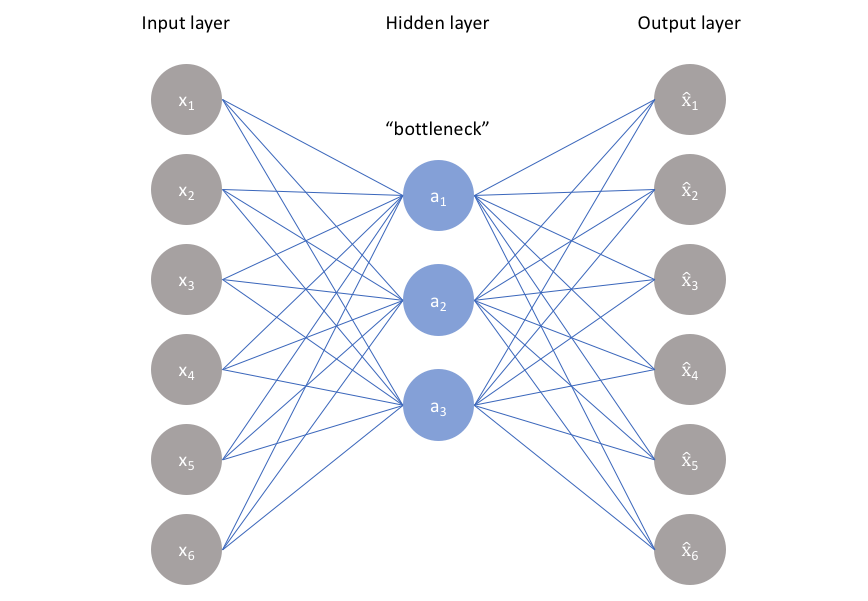
\includegraphics[width=1.0\linewidth]{Chapters/items/autoencoder1.png}
        \caption{}
        \label{fig: auto1}
    \end{subfigure}
    \caption{Bộ mã hóa tự động.}
\end{figure}

\newpage
Nếu các tính năng đầu vào từng độc lập của nhau, việc nén này và tái tạo sau đó sẽ là
một nhiệm vụ rất khó khăn. Tuy nhiên, nếu một số loại cấu trúc tồn tại trong dữ liệu
(ví dụ như: mối tương quan giữa các tính năng đầu vào), cấu trúc này có thể được
học và do đó được tận dụng khi buộc đầu vào thông qua nút thắt cổ chai của mạng.

Bộ mã hóa tự động lý tưởng cân bằng những điều sau đây:
\begin{itemize}[leftmargin=1.5cm]
    \item Nhạy cảm với các yếu tố đầu vào đủ để xây dựng lại một cách chính xác.
    \item Đủ nhạy cảm với các đầu vào mà mô hình không chỉ đơn giản là ghi
          nhớ hoặc trang bị quá nhiều dữ liệu đào tạo.
\end{itemize}

\newpage
Sự đánh đổi này buộc mô hình chỉ duy trì các biến thể trong dữ liệu cần
thiết để cấu trúc lại đầu vào mà không giữ lại các phần dư thừa trong đầu vào.
Đối với hầu hết các trường hợp, điều này liên quan đến việc xây dựng một hàm mất mát
trong đó phải thỏa mãn mô hình của chúng ta nhạy cảm với các yếu tố đầu vào
(ví dụ: xây dựng lại 1 hàm mất mát ${\cal L}\left( {x,\hat x} \right)$ và
thêm một chính quy hóa)


\begin{equation}
    {\cal L}\left( {x,\hat x} \right) + regularizer
\end{equation}

Thông thường, sẽ có thêm một tham số tỷ lệ trước thuật ngữ chính quy để chúng ta
có thể điều chỉnh sự cân bằng giữa hai mục tiêu.

Dưới đây chúng em sẽ trình bày về một số kiến trúc của bộ mã hóa tư động
tiêu chuẩn để áp đặt 2 ràng buộc này và điều chỉnh sự cân bằng.


% \newpage
% \subsection{Cấu trúc bộ mã hóa tự động}
% Một bộ mã hóa tự động có 3 thành phần chính : bộ mã hóa f,
% bộ giải mã g, mô hình xác suất Q

\subsection{Bộ mã hóa tự động chưa hoàn chỉnh}

Kiến trúc đơn giản nhất để xây dựng bộ mã tự động là hạn chế số lượng
nút hiện diện trong (các) lớp ẩn của mạng, hạn chế lượng thông tin có
thể truyền qua mạng. Bằng cách sử dụng các hình phạt mạng theo lỗi xây dựng lại,
mô hình của chúng tôi có thể tìm hiểu các thuộc tính quan trọng nhất của dữ
liệu đầu vào và cách tái tạo tốt nhất dữ liệu đầu vào ban đầu từ trạng thái
"được mã hóa". Lý tưởng nhất là bảng mã này sẽ tìm hiểu và mô tả các thuộc
tính tiềm ẩn của dữ liệu đầu vào.

\begin{figure}
    \begin{subfigure}{0.8\textwidth}
        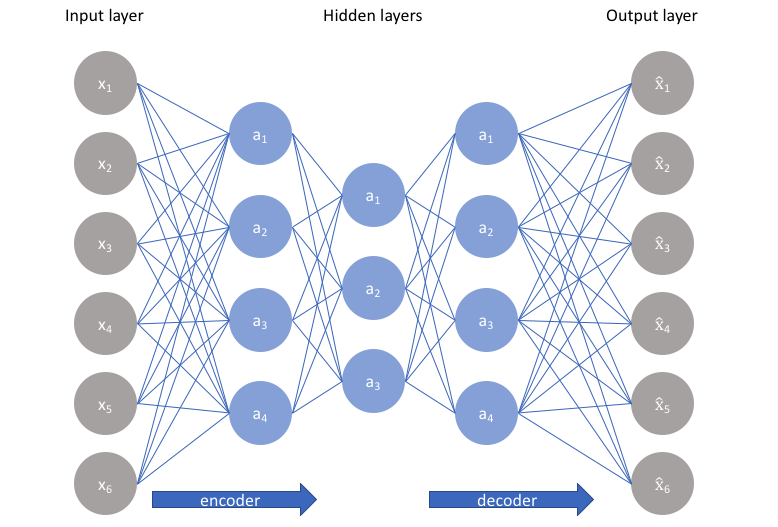
\includegraphics[width=1.\linewidth]{Chapters/items/auto2.jpg}
        \caption{}
        \label{fig: auto2}
    \end{subfigure}
    \caption{Mô tả mô hình bộ mã hóa tự động chưa hoàn chỉnh.}
\end{figure}

Bởi vì mạng nơ-ron có khả năng học các mối quan hệ phi tuyến,
điều này có thể được coi là một sự tổng quát hóa (phi tuyến)
mạnh mẽ hơn của PCA (kĩ thuật giảm chiều dữ liệu tuyến tính)

\newpage
Trong khi PCA cố gắng khám phá một siêu phẳng có chiều thấp hơn
mô tả dữ liệu ban đầu, thì các bộ mã tự động có khả năng học các
đa tạp phi tuyến (đa tạp được định nghĩa theo thuật ngữ đơn giản
là liên tục, không giao nhau bề mặt). Sự khác biệt giữa hai cách
tiếp cận này được hình dung bên dưới.

\begin{figure}
    \begin{subfigure}{0.5\textwidth}
        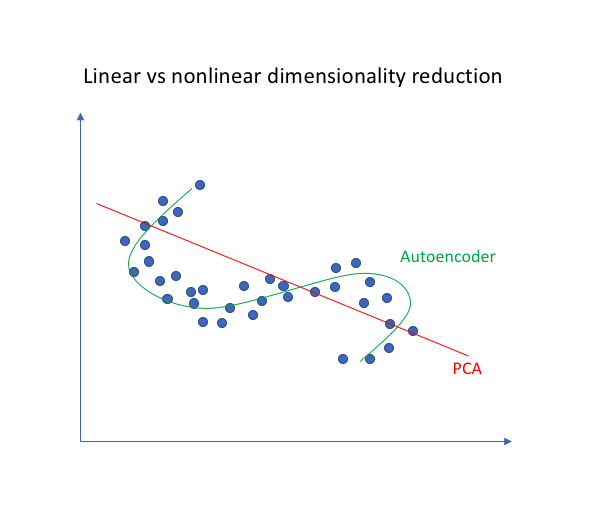
\includegraphics[width=1.\linewidth]{Chapters/items/auto3.jpg}
        \caption{}
        \label{fig: auto3}
    \end{subfigure}
    \caption{Mô tả mô hình bộ mã hóa tự động chưa hoàn chỉnh.}
\end{figure}

Một bộ mã tự động chưa hoàn chỉnh không có thuật ngữ chính quy
rõ ràng - chúng tôi chỉ đào tạo mô hình của mình theo sự mất mát
khi xây dựng lại. Do đó, cách duy nhất của chúng tôi để đảm bảo rằng
mô hình không ghi nhớ dữ liệu đầu vào là đảm bảo rằng chúng tôi đã
hạn chế đủ số lượng các nút trong (các) lớp ẩn.

Đối với các bộ mã tự động sâu, chúng ta cũng phải lưu ý về dung
lượng của bộ mã hóa và các kiểu máy giải mã của chúng ta.
Ngay cả khi "lớp nút cổ chai" chỉ là một nút ẩn, mô hình của
chúng tôi vẫn có thể ghi nhớ dữ liệu huấn luyện với điều kiện là
các mô hình bộ mã hóa và giải mã có đủ khả năng để học một số chức
năng tùy ý có thể ánh xạ dữ liệu thành một chỉ mục.

\subsection{Bộ mã tự động thưa thớt}

Các bộ mã tự động thưa thớt cung cấp cho chúng ta một phương pháp
thay thế để giới thiệu một nút thắt cổ chai thông tin mà không
yêu cầu giảm số lượng nút ở các lớp ẩn của chúng ta. Thay vào đó,
chúng tôi sẽ xây dựng hàm mất mát của chúng tôi để chúng tôi
xử phạt các hàm kích hoạt trong một lớp. Đối với bất kỳ quan sát
nhất định nào, chúng ta sẽ khuyến khích mạng của mình học cách mã hóa và
giải mã chỉ dựa vào việc kích hoạt một số lượng nhỏ nơ-ron.

\begin{figure}
    \begin{subfigure}{0.8\textwidth}
        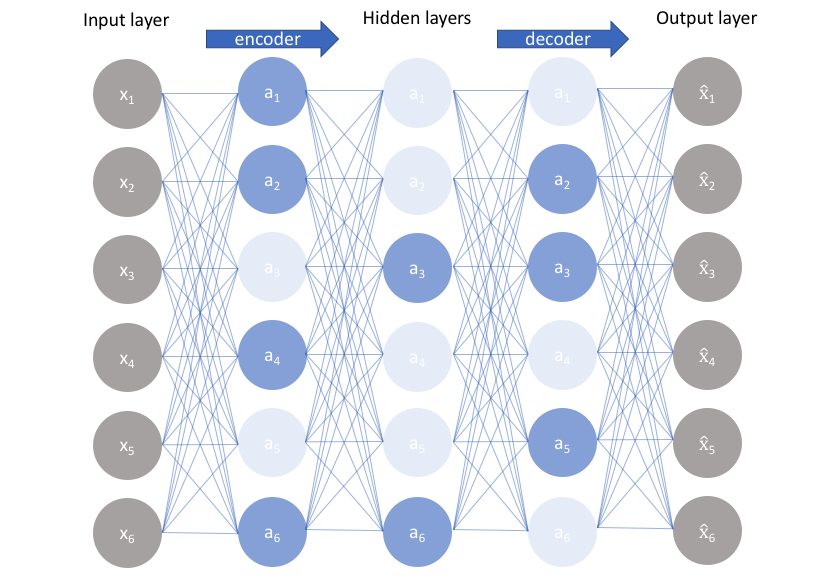
\includegraphics[width=1.\linewidth]{Chapters/items/auto4.jpg}
        \caption{}
        \label{fig: auto4}
    \end{subfigure}
    \caption{Mô tả mô hình bộ mã hóa tự động chưa hoàn chỉnh.}
\end{figure}

\newpage
Một bộ mã tự động thưa thớt chung được hiển thị bên trên nơi
độ mờ của một nút tương ứng với mức độ kích hoạt. Điều quan
trọng cần lưu ý là các nút riêng lẻ của một mô hình được đào
tạo kích hoạt phụ thuộc vào dữ liệu , các đầu vào khác nhau
sẽ dẫn đến việc kích hoạt các nút khác nhau thông qua mạng.

Một kết quả của thực tế này là chúng tôi cho phép mạng của
mình nhạy cảm với các nút lớp ẩn riêng lẻ đối với các thuộc
tính cụ thể của dữ liệu đầu vào. Trong khi một bộ mã tự động
chưa hoàn chỉnh sẽ sử dụng toàn bộ mạng cho mỗi lần quan sát,
một bộ mã tự động thưa thớt sẽ buộc phải kích hoạt có chọn lọc
các vùng của mạng tùy thuộc vào dữ liệu đầu vào. Do đó, chúng
tôi đã giới hạn khả năng ghi nhớ dữ liệu đầu vào của mạng mà
không giới hạn khả năng mạng trích xuất các tính năng từ dữ liệu.

Điều này cho phép chúng tôi xem xét biểu diễn trạng thái tiềm ẩn
và quy định của mạng một cách riêng biệt, do đó chúng tôi có thể
chọn biểu diễn trạng thái tiềm ẩn (tức là kích thước mã hóa) phù
hợp với những gì có ý nghĩa với ngữ cảnh của dữ liệu trong khi áp
đặt chính quy bởi ràng buộc thưa thớt.

Có hai cách chính mà chúng ta có thể áp đặt hạn chế thưa thớt này;
cả hai đều liên quan đến việc đo lường các kích hoạt lớp ẩn
cho mỗi lô đào tạo và thêm một số thuật ngữ vào hàm mất mát để
xử phạt các kích hoạt quá mức. Các cách này là:

\begin{itemize}[leftmargin=1.5cm]
    \item \textbf{L1 Regularization}: Chúng ta có thể thêm một thuật ngữ vào hàm mất mát
          để phạt giá trị tuyệt đối của vector kích hoạt \textit{a} trong lớp \textit{h} với quan sát \textit{i}, được chia tỉ lệ
          bằng 1 tham số điều chỉnh \textit{$\lambda$}
          \begin{equation}
              {\cal L}\left( {x,\hat x} \right) +  \lambda \sum\limits_i {\left| {a_i^{\left( h \right)}} \right|}
          \end{equation}
    \item \textbf{KL-phân kỳ} Về bản chất, KL-phân kỳ là thước đo sự
          khác biệt giữa hai phân phối xác suất. Chúng ta có thể xác định
          tham số thưa thớt \textit{p} biểu thị kích hoạt trung bình của
          một nơ-ron trên một tập hợp các mẫu. Kỳ vọng này có thể được tính là :
          \begin{equation}
              {{\hat \rho }_ j} = \frac{1}{m}\sum\limits_{i} {\left[ {a_i^{\left( h \right)}\left( x \right)} \right]}
          \end{equation}
          trong đó chỉ số con \textit{i} biểu thị nơ-ron cụ thể trong lớp \textit{h}, tính tổng các kích hoạt
          cho các quan sát huấn luyện \textit{m} được ký hiệu riêng lẻ là \textit{x}.

\end{itemize}

\subsection{Bộ mã hóa tự động giảm nhiễu}

Như ở phần giới thiệu, bộ mã hóa tự động chính là một mạng
nơ-ron được đào tạo
trong đó đầu vào giống hệt đầu ra và mô hình có nghiệm vụ tái
tạo đầu vào càng
chặt chẽ càng tốt khi chuyển qua thông tin ở lớp thắt cổ chai.
Một cách tiếp cận khác hướng tới việc phát triển một mô hình
tổng quát hóa là làm nhiễu một chút dữ liệu đầu vào nhưng vẫn
duy trì dữ liệu không bị gián đoạn làm đầu ra mục tiêu của mô hình.

\begin{figure}
    \begin{subfigure}{0.8\textwidth}
        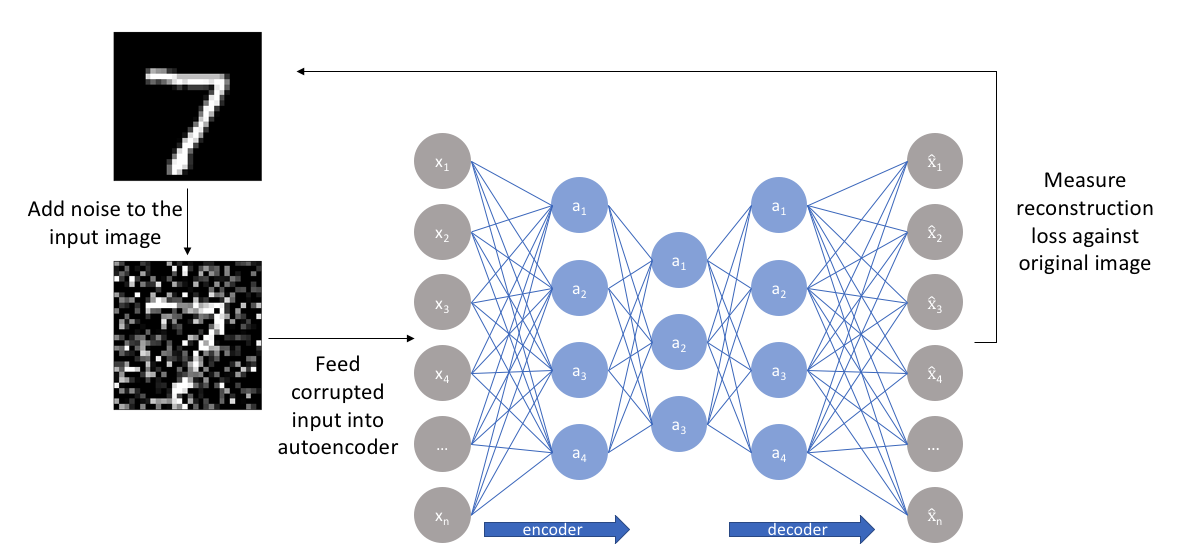
\includegraphics[width=1.\linewidth]{Chapters/items/auto5.jpg}
        \caption{}
        \label{fig: auto5}
    \end{subfigure}
    \caption{Mô tả mô hình bộ mã hóa tự động chưa hoàn chỉnh.}
\end{figure}

Với cách tiếp cận này, mô hình không thể đơn giản
phát triển một ánh xạ ghi nhớ dữ liệu đào tạo vì đầu vào và đầu
ra mục tiêu không còn giống nhau. Thay vào đó, mô
hình học một trường vectơ để ánh xạ dữ liệu đầu vào tới một đa
tạp có chiều thấp hơn (nhớ lại từ hình ảnh trước đây của tôi rằng
một đa tạp mô tả vùng mật độ cao nơi dữ liệu đầu vào tập trung).




